\begin{table}[tb]
\centering\small\setlength{\tabcolsep}{4pt}
\caption{Spline operating policies. Rates are percentages, mean $\pm$ sample SD across five randomizations conditional on each stream. Each threshold uses only past labels.}
\label{tab:costs}
\begin{tabular}{llrrr}\toprule
Stream & Policy & Recall & FPR & BA \\\midrule
\tablerows{tables/diagnostic_a_cost_rows.tex}
\bottomrule\end{tabular}
\end{table}

\begin{table}[tb]
\centering\small\setlength{\tabcolsep}{4pt}
\caption{Requested calibration FPR versus achieved future rates for the spline score. Target and rates are percentages. Mean $\pm$ sample SD describes five randomizations of the same stream. Thresholds use only previously available normal labels.}
\label{tab:fprtargets}
\begin{tabular}{lr l rrr}\toprule
Stream & Target & Controller & Recall & FPR & BA \\\midrule
\tablerows{tables/diagnostic_a_fpr_rows.tex}
\bottomrule\end{tabular}
\end{table}
Figure~\ref{fig:pr} reports precision--recall at the actual causal operating points. TON's attack-dominated prevalence can yield high precision despite a large FPR. To make that dependence visible, the third panel uses the same class-conditional rates at hypothetical 1\% prevalence:
\begin{equation}
 \mathrm{precision}(\pi)=\frac{\pi\,\mathrm{recall}}{\pi\,\mathrm{recall}+(1-\pi)\,\mathrm{FPR}}.
\end{equation}
For example, the TON head at $\lambda=1$ yields 4.37\% precision at 1\% prevalence and 0.45\% at 0.1\%. These are conditional calculations, not predictions for a new network.

\begin{figure}[tb]
\centering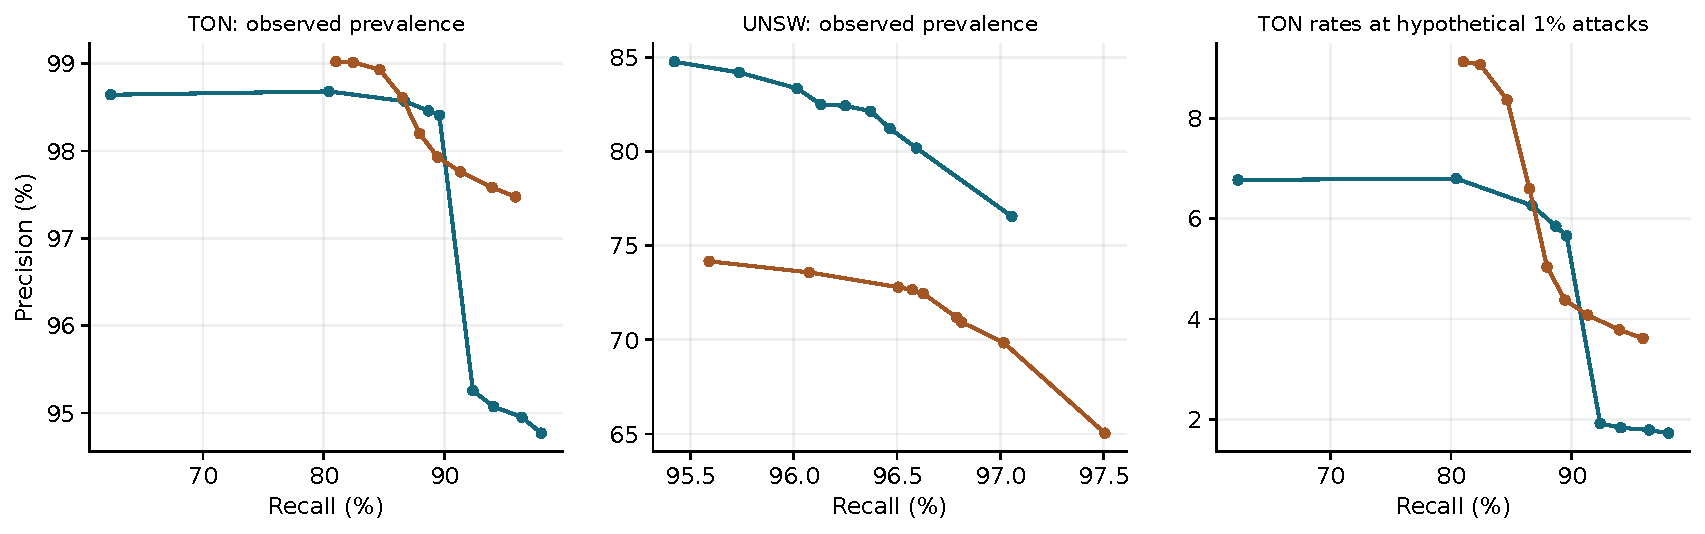
\includegraphics[width=\linewidth]{figures/diagnostic_a_precision_recall.pdf}
\caption{Precision--recall operating points selected by the fixed cost grid. The first two panels use observed class counts. The last panel assumes that TON's class-conditional rates transfer to 1\% attack prevalence. Points are seed means conditional on each capture; they are not pooled adaptive-score PR curves.}
\label{fig:pr}
\Description{Precision--recall operating points selected by the fixed cost grid. The first two panels use observed class counts. The last panel assumes that TON's class-conditional rates transfer to 1\% attack prevalence. Points are seed means conditional on each capture; they are not pooled adaptive-score PR curves.}
\end{figure}

